The input layer is comprised of various sensors, such as the E-stop switch and inductive limit switches. The input layer receives these inputs and directs them to the programmable logic controller for further processing. The host PC is also a component within the input layer, in charge of programming and writing to the system. We can configure the robot arm and the linear rail to execute a task, and in case of an emergency, the E-stop can halt our program instantly.


\subsection{Host PC}
The host PC acts as the centralized component for communication between the robot arm and the PLC. Comprised of software like RTToolbox and GXWorks3, the PC can program the different subsystems to accomplish the application task.

\begin{figure}[h!]
	\centering
 	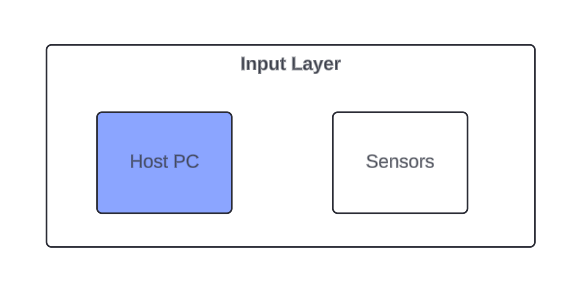
\includegraphics[width=0.60\textwidth]{images/Input_Host.png}
 \caption{Host PC subsystem description diagram.}
\end{figure}

\subsubsection{Assumptions}
Host PC contains all the required software to program the movement of the robot. The program written in host PC will act as an input for our system. 


\subsubsection{Responsibilities}
The program will contain logic behind the specific movement of the robot. The program will be written in a way that the robot only performs a fixed task.


\subsubsection{Subsystem Interfaces}
\begin {table}[H]
\caption {Subsystem interfaces} 
\begin{center}
    \begin{tabular}{ | p{1cm} | p{6cm} | p{3cm} | p{3cm} |}
    \hline
    ID & Description & Inputs & Outputs \\ \hline
    \#01 & Write a robot movement program & \pbox{3cm}{-} & \pbox{3cm}{sends program}  \\ \hline
    \#02 & Write a logic program & \pbox{3cm}{-} & \pbox{3cm}{sends program}  \\ \hline
    \end{tabular}
\end{center}
\end{table}

\subsection{Sensors}
The sensors subsystem consists of emergency stops and inductive limit switches. E-stops serve as a safety feature, allowing users to halt the robot in the event of unexpected actions or when they desire. This sensor can stop the program, regardless of the current processing state. The inductive limit switches act as motion boundaries for the robot and aid with calibration.

\begin{figure}[h!]
	\centering
 	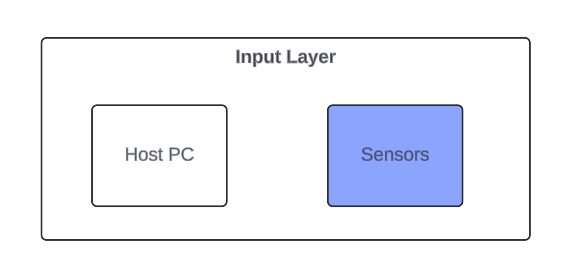
\includegraphics[width=0.60\textwidth]{images/Input_Snsors.png}
 \caption{Sensors subsystem description diagram}
\end{figure}

\subsubsection{Assumptions}
E-stops can be pressed to immediately stop the robot in case of potential collisions, unexpected behavior, or excessive temperature increases. The emergency stops are used in emergency situations, and are not the normal standard for halting robot movement. The inductive limit switches send signals to the robot controller to indicate the robot is reaching its boundary limits. The program written by the PC must include a dynamic calibration sequence that references these limits.

\subsubsection{Responsibilities}
If users press any of the E-stops, the system stops by transmitting the changed input value to the controller. When any of the emergency stop switches are pressed, the switch is closed and the electric signal is outputted, and this value is then relayed to the controller to halt the system. Similarly, any time the robot travels over the limit switch, the contact is closed and sends a signal to the PLC.

\subsubsection{Subsystem Interfaces}

\begin {table}[H]
\caption {Subsystem interfaces} 
\begin{center}
    \begin{tabular}{ | p{1cm} | p{6cm} | p{3cm} | p{3cm} |}
    \hline
    ID & Description & Inputs & Outputs \\ \hline
    \#03 & E-stop signal & \pbox{3cm}{button status} & \pbox{3cm}{closed or open}  \\ \hline
    \#04 & Inductive switches & \pbox{3cm}{closed or open} & \pbox{3cm}{0 or 1}  \\ \hline
    \end{tabular}
\end{center}
\end{table}

% \subsection{Gate}
% The gate sensor is a safety component that detects whether the gate is open or closed.

% \begin{figure}[h!]
% 	\centering
%  	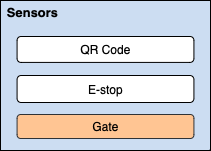
\includegraphics[width=0.60\textwidth]{images/gate.png}
%  \caption{Gate subsystem description diagram}
% \end{figure}

% \subsubsection{Assumptions}
% When the gate is open, the gate sensor sends a 'True' signal to the control, causing the robot to move slowly.

% \subsubsection{Responsibilities}
% Since the gate sensor detects value changes, it must transmit the changed value to the controller for a response.

% \subsubsection{Subsystem Interfaces}
% \begin {table}[H]
% \caption {Subsystem interfaces} 
% \begin{center}
%     \begin{tabular}{ | p{1cm} | p{6cm} | p{3cm} | p{3cm} |}
%     \hline
%     ID & Description & Inputs & Outputs \\ \hline
%     \#03 & Gate open or close & \pbox{3cm}{gate} & \pbox{3cm}{True or False}  \\ \hline
%     \end{tabular}
% \end{center}
% \end{table}

